% File: intro.tex
% Date: Fri Dec 13 17:01:52 2013 +0800
% Author: Yuxin Wu <ppwwyyxxc@gmail.com>

\section{实验目的}
\begin{enumerate}
  \item 实现以16位THCO-MIPS指令集为核心的基础计算机系统
  \item 实现CPU的流水线结构
  \item 能够使用串口和PC进行通信.
\end{enumerate}

\section{实验工具及环境}
\begin{description}
  \item[操作系统] Windows XP (虚拟机)
  \item[软件] Xilinx ISE 14.6
  \item[语言] Verilog
\end{description}

\section{模块设计}
整个系统的模块划分较为复杂.其主要模块如下.
\begin{enumerate}
  \item 主板 \verb|motherBoard.v|: 项目顶层模块,包含整个主板,用于链接外部接口.
  \item 中央处理器 \verb|cpu.v|: 包含了CPU的全部逻辑.
  \item RAM控制器 \verb|memory.v|: RAM的封装.
  \item 串口控制器\verb|serialPort.v|: 串口的封装.
  \item 内存映射器 \verb|memoryMapping.v|: 所有外部存储设备通过其与CPU链接.
  \item 显卡 \verb|graphicCard.v|: 渲染CPU内部信号状态,方便调试.
\end{enumerate}
% TODO: add datapath figure here

\section{实现}
我们实现了基于流水的16位THCO-Mips CPU. 其数据通路架构如下:
\begin{figure}[H]
  \centering
  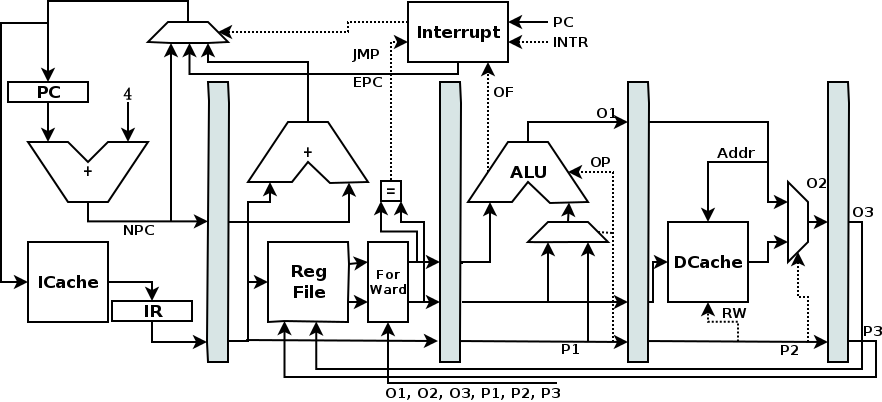
\includegraphics[width=\textwidth]{figure/mips.png}
\end{figure}

\subsection{指令译码}
  CPU顶层通过指令读取模块和指令译码模块进行指令解析, 译码模块
  实现了THCO-Mips 指令集的全部44条CPU指令, 见\verb|instructReader.v, instructDecoder.v|.

  \subsection{读写分离}
<<<<<<< HEAD
    由于每个阶段的输入均是上一阶段的结果,然而在流水作业中,可能某阶段先修改了输出,后一阶段才使用其做为输入。
    为了解决这一问题,将每个时钟周期划分为读入半周期和写出半周期。
    每一阶段在读入半周期时将上一阶段的输出进行读入缓存,然后在输出半周期内使用缓存下来的数据进行写出。
    这样就避免了数据被错误读取的问题。
  \subsection{数据旁路}
    由于流水线的存在,很多时候上一条指令尚未写回时,下一条指令需要使用其做为源寄存器。
    因此从执行阶段和访存阶段引出两条旁路交给译码阶段,如果发现使用的数据被更新但是尚未写回则使用旁路回传的数据而非寄存器堆取出的数据。
    但是无论如何,如果上一条指令是访存指令写入的值永远不能被迅速转。该情况称之为加载延迟,根据MIPS标准可以交由汇编器处理。
  \subsection{跳转}
    跳转指令最快可以在译码阶段才能知道其是否跳转,因此会留下一个被允许的延时槽.
    为了统一跳转指令的行为,以精简设计, 我们在译码阶段将是否跳转解析完毕, 所有的跳转指令都在译码阶段结束时生效,
    因而仅会产生一个延时槽而且不需插入气泡.
  \subsection{存储}
    CPU可能会访问不同的设备,但是不可能为每一个设备定一条CPU指令,因此所有的外设全部被映射到地址的一部分,
    由内存地址映射单元(MMU)来决定对于某内存地址其对应的实际外部设备与其实际物理地址.
    这样对任意外存的访问对CPU而言均是一次对内存的访问.

    在RAM的存储上,由于是流水线的架构,其一条指令需要读写内存两次,在内存资源上会产生结构冲突.
    注意到实际RAM可以进行连续读取,但不能进行连续写入,因此实现中在同一周期的前半段与后半段将会进行两次操作.
    首先进行一次只读操作,然后进行读写操作,可以解决该冲突.
  \subsection{显卡}
    硬件开发一大难点是仿真结果可能和实际结果不一致,虽然仿真可以检查出一部分错误,但是实际综合后可能出现仿真难以发现的问题.
    而在硬件上进行调试不是非常方便,可能需要每次引出不同的信号显示在LED或者数码管上,每次可以监控的信号量有限.
    因此在编写核心代码之前实现了一个显卡,可以方便地将大量信号渲染成为人可读的视觉信号,大大方便了调试.
    %TODO: add vga picture here
  \subsection{中断}
    中断是计算机的一个重要组成部分。为了实现中断,引入了一个新的指令eret,其作用便是从中断处理程序中返回。
    中断分为硬中断和软中断,此次作业中将其进行了分级,硬中断的优先级高于软中断。
    处理时首先由中断仲裁器决定触发哪一个中断,中断处理器查看是否可以触发中断。
    如果可以则会记录当前的PC值与取指令阶段取出的指令,修改PC值为中断处理程序入口,设置中断屏蔽位,并将气泡(nop)传给译码阶段。
    在接收到eret指令时,中断处理器将PC还原,恢复中断屏蔽位,并无视取出的指令,把之前存储的指令交给译码阶段继续执行。
    因此中断触发int和返回指令eret均无延时槽。
    触发中断时引入的气泡也是本项目中唯一可能引入的气泡。

\section{实验结果}
  最终实现的版本有两个.
  \subsection{目标分支}
    期望目标是运行带线程切换的文本编辑器与简单脚本语言解释器,但是由于硬中断的实现时间太晚,没有足够的时间基于其继续开发,因此停留在将输入数据载入I/O缓存区,虽然编写了文本编辑器和解释器但是没有时间进行调试.
  \subsection{基础分支}
    基础分支实现了串口,能够正确高效地与监控程序进行通信,可以运行自己汇编编写的所有程序,实现了实验的基本要求.

\section{经验及总结}
  此次实验中出现了很多问题,最后大多得以解决.
  \subsection{中断}
    由于设计时未想清楚,将硬中断当作跳转指令处理,而没有考虑插入时读入了一个跳转指令,导致程序出现不稳定错误.
    后来在随机仿真测试中才发现该问题.
  \subsection{RAM访问}
    手动时钟测试没有问题之后,将CPU时钟定为50M,发现对RAM的写入存在问题,反复多次调试无果后注意到RAM的最短数据保持时间,将时钟降为25M后获得成功.
  \subsection{链接错误}
    曾经出现过莫名的错误,调试逻辑半天无果后打开了RTL图,发现一个调试信号输出删除后,其父模块的链接表中却依然保留,使得出现在其之后的信号全部错位,修复后问题解决。
  \subsection{汇编器}
    在调试中为了测试更多的代码需要写一些复杂的程序.
    而给出的汇编器仅仅对汇编指令做了机械的翻译,因此实现了一个支持伪指令的汇编器,
    可以将伪指令如if等翻译成CPU指令,减少了编写复杂程序出现的bug的机会.
    %TODO: add assembler example here
  \subsection{版本控制}
    采用git做为版本控制手段.
    由于监控程序没有TLB,而且需要串口通信,与最终预期目标存在较大的冲突,因此在完成基础部分之后分裂为master和basic两个分支进行开发.
    master分支实现了PS/2键盘和软硬中断以及显存原型,而basic分支无中断而是增加了串口通信,两部分互不干扰,切换也十分方便.
    使用git也能够保存每个版本的信息,方便进行回滚和比较.
    %TODO: add git log graph here

    此外,使用git也使得合作开发更为便利.其他同学开发的汇编器、预处理器等代码也能够方便的进行同步,特别是小组三人分处三个寝室,面对面交流不便,在代码交换与同步方面节省了大量的时间.

\section{一些建议}
  在指令集中需要添加两条指令,一条是从中断中返回的指令eret,另一条是从栈中取到ra寄存器的指令lw_rs。
  目前的指令集中没有中断处理返回的指令,导致无法完成中断的功能。
  而且目前的指令集唯一能够写入ra寄存器的是jalr,而且被写入ra的值和PC有关,在该指令集下无法编写递归程序,或者函数调用嵌套程序。

  此外,根据MIPS标准,0号寄存器的值应当一直为0,会忽视一切对其值进行写入的指令,但是kernel中对0号寄存器写入并使用了非0值,与标准不符。


